%%% Version 4.4 Generated 2018/06/15 %%%
\documentclass[utf8]{FrontiersinHarvard}
\usepackage{url, hyperref, lineno, microtype}
\usepackage[onehalfspacing]{setspace}

\usepackage{multirow}
\usepackage{xspace}
\usepackage{siunitx}
\usepackage[version=4]{mhchem}
\usepackage{textcomp} % registered trademark and copyright symbols
\usepackage{graphicx, subcaption}

% See mode, number-mode and unit-mode; values are text, math, and match
\sisetup{separate-uncertainty=true, 
    exponent-product=\cdot,
    per-mode=symbol,
    mode = text,
    range-units=single}
\DeclareSIUnit{\year}{yr}
\graphicspath{{"figures/"}}

% \linenumbers
\def\keyFont{\fontsize{8}{11}\helveticabold }

% Set author information
% --------------------------------------------- %
\def\firstAuthorLast{Sample {et~al.}}
\def\Authors{Mastnak, Elijan J.\,$^{1,*}$, Djordević, Srdjan\,$^{2}$, Krašna, Simon\,$^{3}$ and TO-DO who else?}
\def\Address{$^{1}$University of Ljubljana, Faculty of Mathematics and Physics, Ljubljana, Slovenia. elijan-jakob.mastnak@student.fmf.uni-lj.si \\
$^{2}$TMG-BMC Ltd., Štihova ulica 24, 1000 Ljubljana, Slovenia. srdjand@tmg.si \\
$^{3}$University of Ljubljana, Faculty of Mechanical Engineering, Ljubljana, Slovenia. simon.krasna@fs.uni-lj.si}
\def\corrAuthor{Sample}
\def\corrEmail{sample@provider.com}
% \def\corrAuthor{Elijan Mastnak}
% \def\corrEmail{elijan-jakob.mastnak@student.fmf.uni-lj.si}
% --------------------------------------------- %

% Define custom macros
% --------------------------------------------- %
\newcommand{\TODO}[1]{{\textbf{TODO:} {\color{red} #1}}}

% TMG parameters
% --------------------------------------------- %
\newcommand{\Dm}{\ensuremath{\text{Dm}}\xspace}
\newcommand{\Td}{\ensuremath{\text{Td}}\xspace}
\newcommand{\Tc}{\ensuremath{\text{Tc}}\xspace}
\newcommand{\RDDMax}{\ensuremath{ \text{RDD}_{\text{max}}}\xspace}
\newcommand{\RDDMaxTime}{\ensuremath{ \text{TRDD}_{\text{max}}}\xspace}
% --------------------------------------------- %

% SPM parameters
% --------------------------------------------- %
\newcommand{\SPMStart}{\ensuremath{\text{SPMStartTime}}\xspace}
\newcommand{\SPMEnd}{\ensuremath{\text{SPMEndTime}}\xspace}
\newcommand{\SPMCentroidTime}{\ensuremath{\text{SPMCentroidTime}}\xspace}
\newcommand{\SPMCentroidT}{\ensuremath{\text{SPMCentroid}}\xspace}
\newcommand{\SPMMax}{\ensuremath{\text{SPMMax}}\xspace}
\newcommand{\SPMArea}{\ensuremath{\text{SPMArea}}\xspace}
% --------------------------------------------- %

\begin{document}
\onecolumn
\firstpage{1}

\title[Quantifying Twitch Potentiation with TMG and SPM]{Quantifying Post-Activation Twitch Potentiation with Tensiomyography and Statistical Parametric Mapping} 

\author[\firstAuthorLast ]{\Authors}
\address{}
\correspondance{}
\extraAuth{}

\maketitle

% The abstract should render the general significance and conceptual advance of the work clearly accessible to a broad readership.
\begin{abstract}
\section{}
This study proposes and demonstrates in practice the use of statistical parametric mapping for reliably detecting and quantifying post-activation twitch potentiation in superficial skeletal muscles.
The study applies SPM to tensiomyographic measurements of the rectus femoris muscle's contractile response during electrically-induced twitch contraction following an incline squat conditioning exercise. SPM was found to reliably and quantitatively differentiate between the muscle's pre-conditioning and post-conditioning response, indicating the presence of post-activation potentiation.
More so, because SPM preserves the time-domain information contained in the original muscle response, SPM also gives an indication of \textit{when} the potentiation-like state occurred over the course of the muscle twitch.

\tiny
\keyFont{\section{Keywords:} tensiomyography, statistical parametric mapping, twitch potentiation, post-activation potentiation, neuromuscular electrical stimulation}
% Provide 5-8 keywords
\end{abstract}

\section{Introduction}
In the phenomenon generally called post-activation potentiation, a short, intense burst of muscle activity (called a \textit{conditioning exercise} in this context) temporarily increases the amplitude, force, and speed of both voluntary and electrically induced muscle contractions that immediately follow \citep{brown, oleary, blazevich, mccann, skurvydas}.

In general, prior muscle activity produces two different---and potentially coexistent---muscle responses: fatigue and potentiation.
Limited by the inevitable onset of fatigue, one cannot use conditioning exercises to increase subsequent muscle performance via potentiation ad infinitum---eventually fatigue outweighs any potentiation-like performance improvement.
Fatigue can coexist with PAP \citep{rassier}, and measured muscular performance represents the net balance between processes that cause fatigue and processes that cause potentiation \citep{rassier}.
Striking a favorable balance between fatigue and potentiation should be of interest to coaches, sports scientists, and athletes alike.
Doing so requires a reliable means of detecting and quantifying potentiation, and this article offers a novel way of doing so---directly in the time domain in which the muscle response is originally measured.

\subsection{On PAP, PAPE, and twitch potentiation}
We pause briefly to comment on some ambiguity in the literature surrounding post-conditioning enhancements in muscular performance,
generally involving confusion between the following two phenomena \citep{prieske}.
\begin{itemize}

    \item \textit{Post-activation potentiation} (PAP) is a short-term enhancement in a muscle's contractile properties during an electrically-induced muscle twitch, which generally manifests as enhanced twitch force and amplitude, and decreased time to peak contraction.
    PAP has a short half-life ($ \sim \SI{30}{\second} $; \cite{vandervoort}),
    is verified at the specific level of an individual muscle using a non-voluntary, electrically-induced muscle twitch, and generally requires nontrivial equipment and a standardized test environment to measure.

    \item \textit{Post-activation performance enhancement} (PAPE) is
    a somewhat longer-term performance improvement in exercises serving as measures of maximal strength, power, and speed (e.g. a maximum vertical jump or a 60-meter sprint).
    PAPE has a longer half-life (maximum performance enhancement occurs on the order of 5 to 10 minutes following the initial conditioning exercise; \cite{wilson}),
    is verified at a macroscopic level by observing exercise performance (rather than measuring the contractile properties of a specific muscle),
    and is thus simpler to measure than than PAP, possibly at the expense of a less controlled and systematic experiment.

\end{itemize}

The present study concerns PAP, i.e. the short-term, post-conditioning enhancement in muscular contractile properties during electrically-induced twitch, and for this reason we will tend to use the more specific term \textit{twitch potentiation}.
Borrowing the definition of \cite{hodgson},
``a twitch is a brief muscle contraction in response to a single presynaptic action potential or a single, synchronised volley of action potentials.''
Twitch potentiation (TP) is a well-established and reproducible phenomenon that manifests as both enhanced muscle twitch amplitude \citep{gossen, hamada, vandervoort} and decreased time to attaining maximum amplitude \citep{sasaki, sale, grange}.

TP has been demonstrated using electrically induced twitch contractions and attributed to phosphorylation of myosin regulatory light chains \citep{grange}, which makes actin and myosin more sensitive to \ce{Ca^2+} ions \citep{hodgson}.
The muscle's potentiated state has also been attributed to an increase in $ \alpha $-motoneuron excitability \citep{mccann}.
Fatigue induces a decrease in amplitude and velocity of twitch contraction, while PAP causes an increase in amplitude and velocity of twitch contraction and thus enhanced contractile response \citep{hodgson, rodriguez-falces, sasaki}.

\subsection{Quantifying potentiation}
Currently, it is standard to quantify the level of twitch potentiation using discrete twitch contraction parameters computed retrospectively from measurements of muscle displacement, force production, or electrical activity with respect to time.
Examples of these parameters include maximal amplitude of muscle contraction, time taken to reach peak contraction, maximal twitch rate of force development \citep{cochrane, kuu, wallace}, and peak M-wave amplitude \citep{rodriguez-falces}.
In each case, computing these parameters reduces the originally-measured muscle response, which is generally a one-dimensional time series (e.g. muscle displacement with respect to time), to a single number, i.e. a zero-dimensional scalar value.
One can then compare pre-conditioning and post-conditioning parameter values to retrospectively infer the presence (or lack) of post-activation potentiation.

A promising new approach to quantifying TP would analyze 
muscle response and detect and quantify potentiation directly in the time domain in which the muscle response was originally measured, without the dimensionality reduction imposed by computing discrete twitch contraction parameters.
One way of performing such an analysis is the method of statistical parametric mapping (SPM) \citep{friston, pataky-spm1d, pataky-roi, pataky}.

Borrowing the definition of \cite{flandin},
``Statistical parametric mapping is the application of random field theory to make inferences about the topological features of statistical processes that are continuous functions of space or time''.
SPM has so far found its greatest application in neuroimaging for detecting regionally-specific brain activations \citep{friston}.
We use SPM similarly in the present study---applied to one-dimensional functions of time (i.e. twitch amplitude with respect to time) instead of three-dimensional functions of space (i.e. brain scans)---to detect regionally-specific differences between pre-conditioning and post-conditioning muscle responses directly in the time domain.
Statistically significant differences between pre-conditioning and post-conditioning muscle responses are then interpreted as post-activation potentiation.
Most promisingly, because SPM preserves the time-domain information contained in the original muscle response, SPM gives an indication of \textit{when} the potentiation-like state occurred over the course of the muscle twitch.
Of course SPM and conventional twitch contraction parameters can be used together as a means of detection potentiation---there is no need for the to methods to be mutually exclusive.

Quantifying twitch potentiation, then, requires two things: a means of measuring a muscle's contractile response following a conditioning exercise and a technique for analyzing the measured muscle response that can determine the presence (or lack) of potentiation.
Tensiomyography (TMG) is a standard method for selectively measuring contractile response and assessing twitch contraction parameters in superficial skeletal muscles \citep{valencic, dahmane-fiber, dahmane-measurement, meglic, simunic, martin-rodriguez, ce}.
This study assessed TP in a sports training setting by analyzing TMG measurements of electrically-induced muscle contraction both
\begin{enumerate}

    \item using SPM applied directly to TMG muscle responses in the time domain, and

    \item using discrete (zero-dimensional) TP parameters, computed retrospectively from the measured TMG signal, that summarize the muscle's twitch contraction properties.

\end{enumerate}
The study aimed to find if TMG measurement of muscle response followed by SPM analysis of this response can accurately and consistently identify statistically significant differences in the pre- and post-conditioning contractile response of the rectus femoris muscle, and,
if yes, to identify and quantify the associated time-domain changes of twitch potentiation.

\section{Materials and Methods}
\subsection{Participants}
The present study analyzed 54 subjects (age \SI{28.17 \pm 10.9}{\year}; height \SI{178.15 \pm 10.43}{\centi \meter}; weight \SI{71.84 \pm 12.82}{\kilogram}; 28 male and 26 female; 37 elite athletes and 17 recreational).
% TODO describe the simple random random sampling strategy?
To be approved for participation, subjects were required to be injury-free at the beginning of the testing protocol.
The intention and experimental procedure was described to all subjects, and written informed consent was obtained.
The investigation was approved by the Institutional Research Ethics Committee (University of Belgrade, Faculty of Sport and Physical Education), following the recommendations of the Declaration of Helsinki.

\subsection{Study Design}

\subsubsection{Tensiomyography specifications}
The study used tensiomyograhy (TMG) to measure the pre-conditioning and post-conditioning contractile responses of the rectus femoris (RF) muscle.
TMG measurements were taken with the TMG S1 measurement system (TMG-BMC, Ljubljana, Slovenia), which uses an opto-inductive sensor with a spring of spring constant \SI{0.17}{\newton \per \milli \meter} that generates an initial pressure of approximately \SI{1.5e-2}{\newton \per \milli \meter \squared} on a tip area of \SI{11.34}{\milli \meter \squared}.
Two self-adhesive electrodes (UltraStim\textregistered{} Wire, Axelgaard, USA) were positioned approximately along the anatomical axis of the femur, proximal on the beginning of RF and distal \SI{10}{\centi \meter} apart \citep{maffulietti}, symmetrically \SI{2}{\centi \meter} from the sensor on the RF muscle.
The positive electrode (anode) was placed proximally, and the negative electrode (cathode) distally, as shown in Figure~~\ref{fig:electrodes}.

\begin{figure}
	\centering
    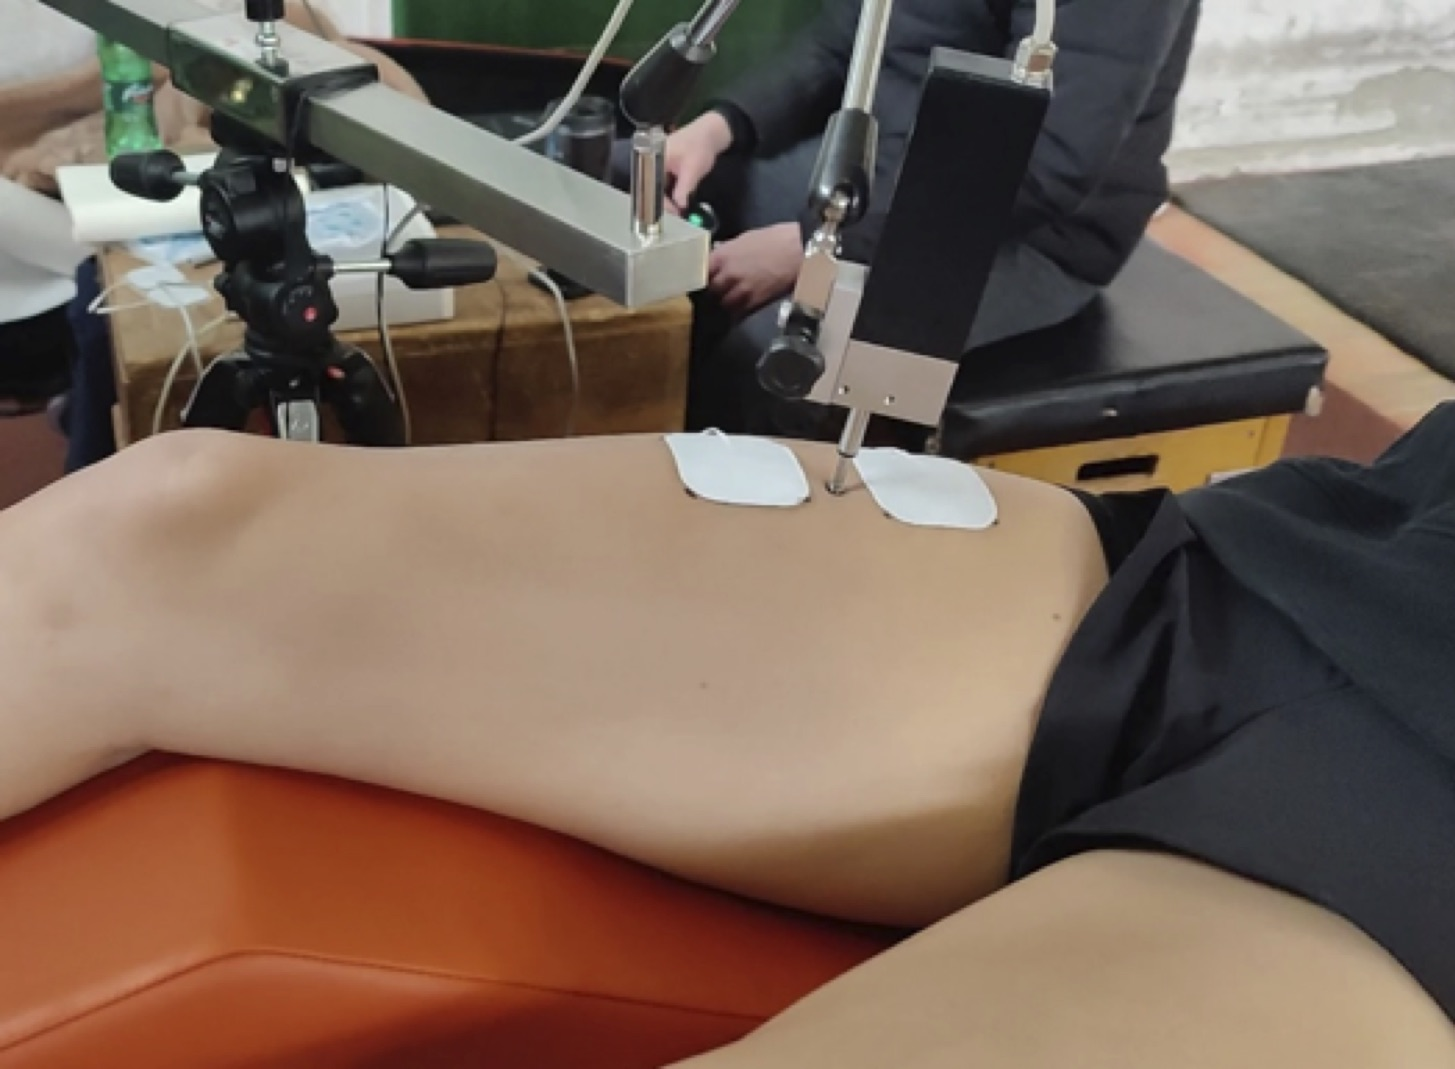
\includegraphics[width=0.65\textwidth]{electrodes.jpg}
    \caption{The position of the electrodes used for electrical muscle simulation.}
    \label{fig:electrodes}
\end{figure}

The electrodes remained fixed on the skin for the duration of the measurement and exercise procedure.
The sensor tip's position on the rectus femoris muscle was marked for reference at the beginning of the measurement protocol, and the same tip position was used for all measurements.
A single-twitch electrical stimulus (a DC pulse of \SI{1}{\milli \second} duration) induced an isometric muscle contraction,
and the muscle response was recorded and analyzed using a standardized algorithm for the TMG S1 system.
A typical TMG signal, along with the standard twitch contraction parameters computed from it, is shown in Figure~\ref{fig:tmg_example}.

\begin{figure}
	\centering
    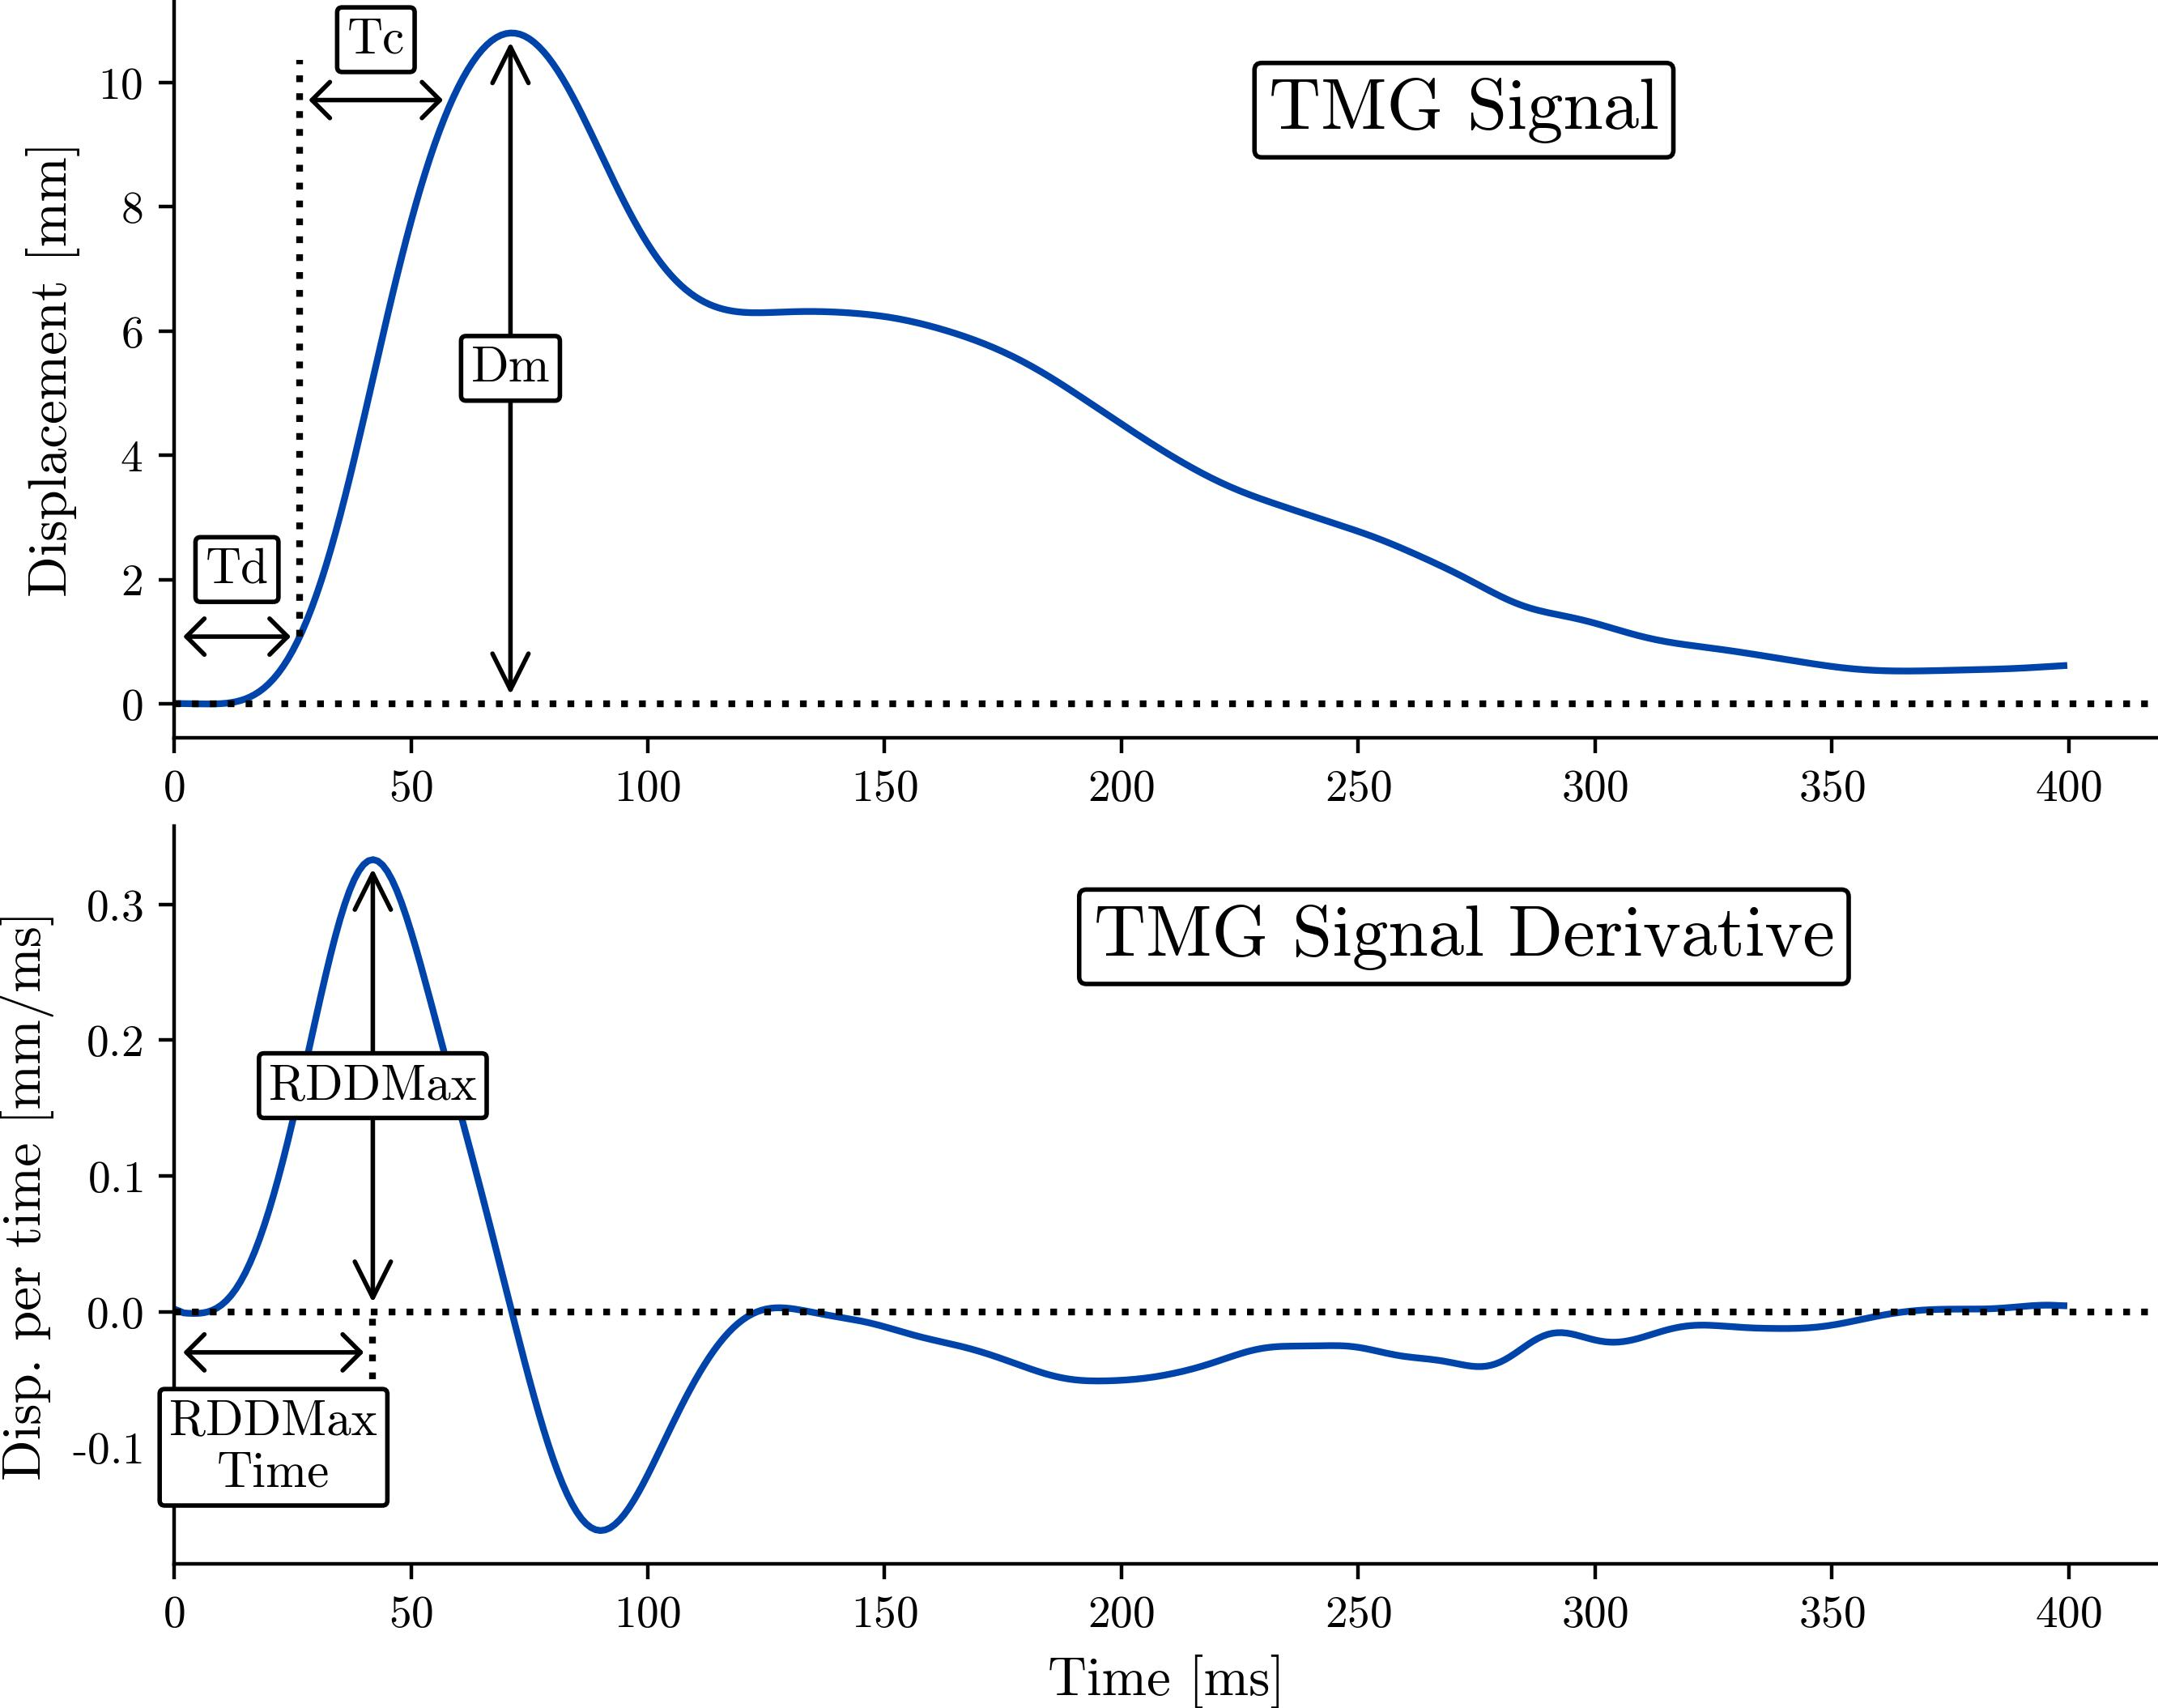
\includegraphics[width=0.95\textwidth]{tmg-example.jpg}
    \caption{A representative TMG signal (top) and its derivative with respect to time (bottom), together with the discrete twitch contraction parameters used to summarize these signals.
    The TMG signal measures the muscle belly's displacement over the course of an electrically-induced twitch contraction;
    RDD stands for rate of displacement development, in analogy with RFD for rate of force development.}
    \label{fig:tmg_example}
\end{figure}

The electrical stimulation intensity applied to the rectus femoris muscle was increased using the standard TMG protocol \citep{valencic, dahmane-fiber, dahmane-measurement}.
After each twitch electrical stimulus, the electrical current was increased until the muscle reached supramaximal response;
the electrical current level for supramaximal muscle response was then used for electrical stimulation in all subsequent measurements.

\subsubsection{Conditioning Exercise}
The study used a weighted incline squat (ISQ) as the conditioning exercise intended to activate a potentiated muscle state. 
The volunteers performed the ISQ on a platform with a slope angle of $ \ang{30} $, holding an additional load of between $ \SI[parse-numbers = false, mode = match]{2 \times 0}{\kilogram} $ and $ \SI[parse-numbers = false, mode = match]{2 \times 20}{\kilogram} $ in each hand (Figure~\ref{fig:isq});
the load was chosen based on a ten-repetition maximum test performed the day before.
The knee angle ranged from $ \ang{0} $ to $ \ang{90} $, while the torso-femur angle remained constant at $ \ang{0} $ throughout the movement.
% TODO figure 4a and 4b
The squat was performed with precise timing for all volunteers: \SI{1}{\second} going down (i.e. from a knee angle of $ \ang{0} $ to $ \ang{90} $) and \SI{1}{\second} coming up (i.e. from a knee angle of $ \ang{90} $ to $ \ang{0} $); a metronome kept time.

\begin{figure}
	\centering
    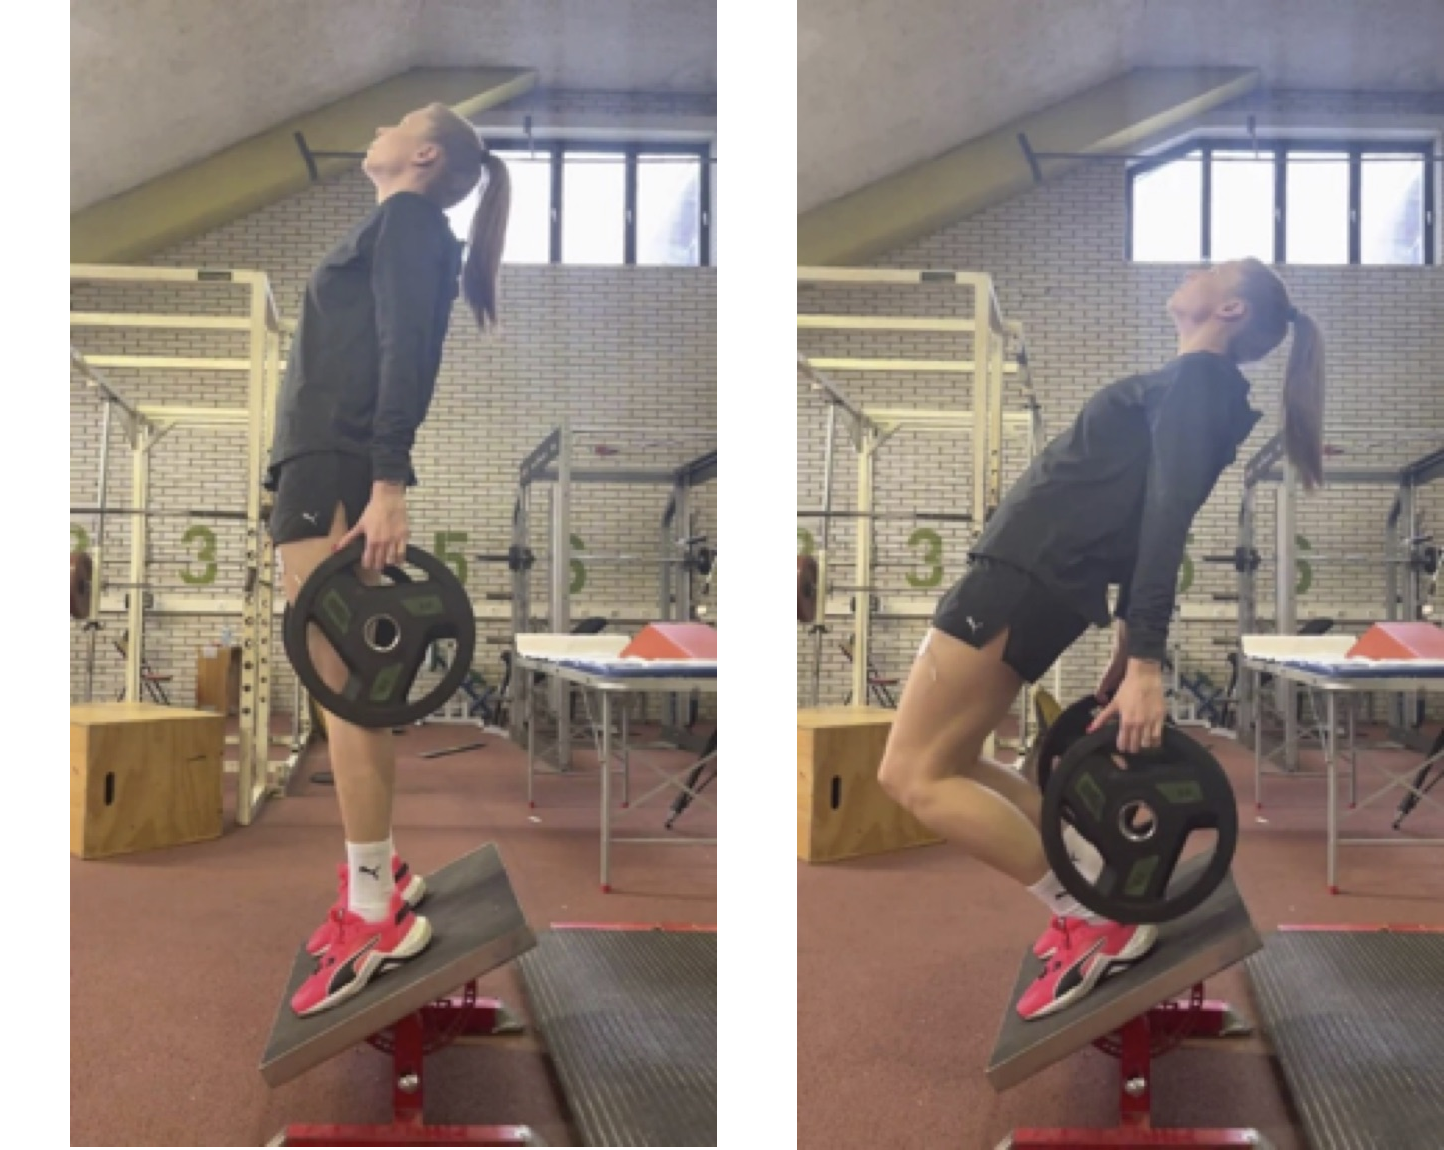
\includegraphics[width=0.65\textwidth]{isq.png}
    \caption{The incline squat used as the conditioning exercise in this study.}
    \label{fig:isq}
\end{figure}

\subsubsection{Measurement Protocol} \label{sss:measurement_protocol}
The study used the following conditioning exercise and TMG measurement protocol:
\begin{enumerate}

    \item pre-conditioning (baseline) TMG measurement(s), followed within \SI{15}{\second} by...

    \item eight repetitions of ISQ, followed within \SI{12}{\second} by...

    \item post-conditioning TMG measurement(s), followed by...

    \item a rest period of \SI{150}{\second}.

\end{enumerate}
This four-step procedure is shown in Figure~\ref{fig:protocol} and was repeated eight times by each subject.
For subjects 1-16, eight pre-ISQ and eight post-ISQ TMG measurements were taken in rapid succession (less than \SI{1}{\second} between successive measurements) in each of the eight measurement sets, for a total of 64 pre-ISQ and 64 post-ISQ TMG measurements per subject.
For subjects 17-54, one pre-ISQ and one post-ISQ TMG measurement was taken in each measurement set, for a total of 8 pre-ISQ and 8 post-ISQ TMG measurements per subject.
The rationale for taking multiple measurements is to generate large enough sample sizes for sufficient statistical power in hypothesis tests comparing pre-ISQ and post-ISQ muscle properties.

\begin{figure}
	\centering
    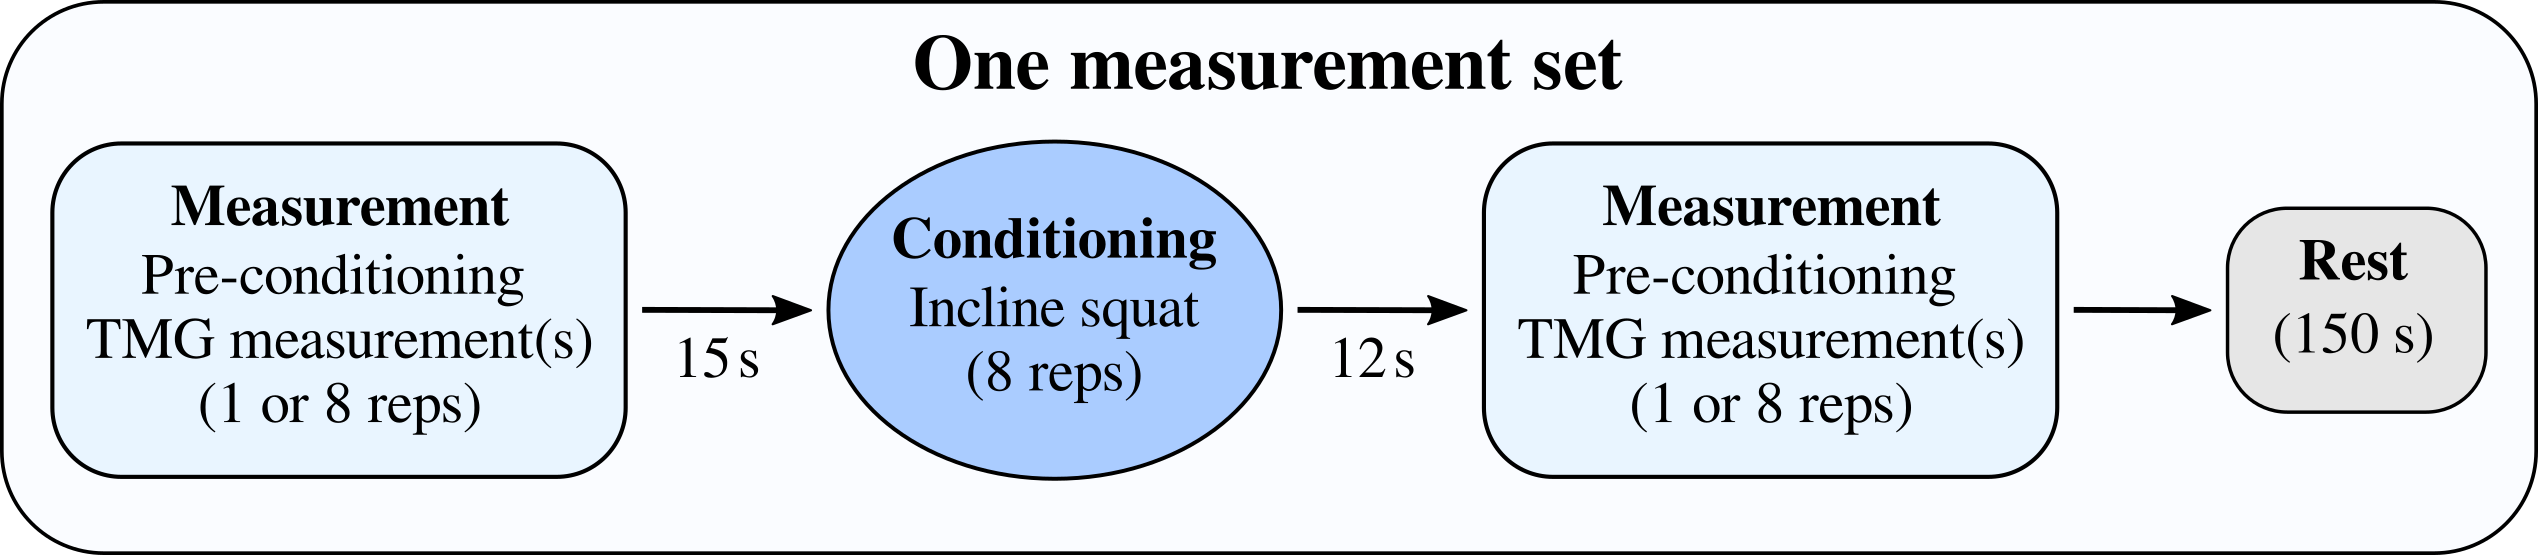
\includegraphics[width=\textwidth]{protocol-set.png}
    \caption{One set of the conditioning exercise and measurement protocol used in the study.
    One such measurement set was repeated eight times by each participant over the course of the testing protocol.
    Eight pre-ISQ and eight post-ISQ TMG measurements were taken per set for subjects 1-16, while one pre-ISQ and one post-ISQ TMG measurement was taken per set for subjects 17-54.}
    \label{fig:protocol}
\end{figure}

\subsubsection{Estimated Load on the Quadriceps Muscle}
An inverse dynamics analysis of a three-segment planar human body model, assuming a quasi-static condition (see Appendix 1) \citep{yoshioka, fry, hof}, was used to estimate the load on the quadriceps muscles (especially the RF, which is loaded at the full amplitude of knee movement) during the ISQ.
The model's body segment properties were estimated using anthropometric data and the subject’s body height and body mass as input parameters \citep{winter}.
% TODO: clarify with the anthropometric data is. Is this the distance from knee to foot?
The subjects' motion in the sagittal plane was recorded on video, and one exercise repetition was selected for estimating the inter-segmental angles (Figure 4).
The peak value of the net knee joint moment was estimated at the lowest body position in the ISQ,
and normalized to the volunteer’s body mass to reduce the effect of inter-subject variance \citep{wannop, moiso}.
The normalized peak values of the knee joint moment were used to compare the loading of the knee extensor muscles during the ISQ between the volunteers.

\subsection{Analysis of Muscle Contractile Response} \label{ss:analysis}

\subsubsection{Software}
Data analysis and standard statistical tests were performed in the Python 3 programming language (\url{https://www.python.org/}) using the Numpy and SciPy libraries (\url{https://numpy.org/}, \url{https://scipy.org/});
and with SPSS Statistics 20 (SPSS Inc., Chicago, IL, USA) and Microsoft Excel.
Statistical parametric mapping analysis was performed in Python 3 using the SPM1d library \citep{pataky-spm1d}; \url{https://www.spm1d.org}.

\subsubsection{Discrete Twitch Contraction Parameters} \label{sss:discrete_twitch_params}
The RF's contractile response was measured with TMG, which records muscle belly displacement with respect to time over the course of the muscle twitch.
The signal is sampled for \SI{1}{\second} at a sample rate of \SI{1}{\kilo \hertz}, for a total of 1000 data points.
A typical TMG signal and its time derivative are shown in Figure~\ref{fig:tmg_example}.
The TMG derivative was computed with a finite difference scheme using the Numpy library's \texttt{gradient} function with a time-spacing of \SI{1}{\milli \second} between data points;
the \texttt{gradient} function uses second-order finite differences at central points and a first-order one-sided forward (backward) finite difference at the left (right) endpoint.
The following five discrete twitch contraction parameters were computed from every measured TMG signal.
\begin{enumerate}

    \item \Dm: maximum displacement of the muscle belly during contraction;
    % (typical values fall in the range \SIrange{6}{12}{\milli \meter});

    \item \Td (delay time): time taken for muscle belly displacement to reach 10 percent of its maximum value;
    % (typical values fall in the range \SIrange{20}{26}{\milli \second});

    \item \Tc (contraction time): time taken for muscle belly displacement to change from 10 to 90 percent of its maximum value;
    % (typical values fall in the range \SIrange{22}{34}{\milli \second});

    \item \RDDMax (maximum rate of displacement development): the maximum rate of change of muscle belly displacement with respect to time, i.e. the maximum value of the TMG signal's time derivative;
    % (typical values fall in the range \SIrange{0.25}{0.40}{\milli \meter \per \milli \second});

    \item \RDDMaxTime: the time at which the TMG signal's time derivative attains its maximum value, i.e. the time at which \RDDMax occurs.
    % (typical values fall in the range \SIrange{30}{45}{\milli \second});

\end{enumerate}
Each of these parameters is marked in Figure~\ref{fig:tmg_example}.
To estimate post-activation potentiation, the five above-described twitch contraction parameters were computed for every TMG measurement for all subjects.
The pairwise differences in pre- and post-conditioning parameter values then served as indicators of potentiation.

\subsubsection{Statistical testing of discrete contraction parameters} \label{sss:discrete_twitch_param_stats}
Broadly speaking, one identifies post-activation potentiation by comparing pre- and post-conditioning parameter values:
appreciably larger values of \Dm (indicating larger twitch amplitude) and \RDDMax (indicating greater rate of force development), and appreciably smaller values of \Td, \Tc, and \RDDMaxTime (indicating a faster muscle response) in the post-conditioning response relative to the pre-conditioning response indicate post-activation twitch potentiation.

For each of the five twitch contraction parameters, we assume the null hypothesis that pre- and post-conditioning parameter values were drawn from populations with the same mean
(interpreted more loosely, that any difference in pre- and post-conditioning values is due to chance alone and there is no meaningful difference in pre- and post-conditioning contraction properties)
and then test this hypothesis with a paired Student's $ t $-test.

Statistical testing imposes an important challenge:
any binary hypothesis test must act on a large-enough sample size to have meaningful statistical power (i.e. probability of correctly rejecting the null hypothesis).
In the context of this study, this means any Student's $ t $-test comparing pre- and post-ISQ parameter values must act on a sample of \textit{many} pre- and post-ISQ pairs; comparing only one pre-ISQ and one post-ISQ value would be statistically meaningless.
There is no exact answer on what sample size is ``large enough''; we use at least eight (pre-ISQ, post-ISQ) pairs for all hypothesis tests in this study, while five pairs might serve as a tentative lower bound.
We considered the following three ways of constructing testable (pre-ISQ, post-ISQ) pairs for each of the five twitch contraction parameters mentioned in Section~\ref{sss:discrete_twitch_params}:
\begin{enumerate}

    \item For subjects 1-16, for whom 8 pre-ISQ and 8 post-ISQ TMG measurements were taken in each measurement set, we compare all 8 pre-ISQ parameter values from a given measurement set against all 8 post-ISQ parameter values from the same set.
    This test would be used in practice to test for potentiation in a given subject after a single conditioning exercise set, and is probably the most useful for practical analysis of PAP.

    \item For subjects 17-54, for whom 1 pre-ISQ and 1 post-ISQ TMG measurement was taken per measurement set, we compare the 8 total pre-ISQ parameter values (one from each of the 8 measurement sets) to the corresponding 8 post-ISQ parameter values.
    We perform a similar cross-set comparison for subjects 1-16, using only the first pre-ISQ and first post-ISQ TMG measurement per set, again for a total of 8 (pre-ISQ, post-ISQ) pairs per subject.
    This test captures a subject's muscle response over the entire 8-set measurement protocol, and gives an indication of the extent to which the subject consistently produced a potentiation-like state in each exercise set over the course of the entire testing protocol.

    \item For each measurement set, we compare all subjects' pre-ISQ parameter value to the corresponding post-ISQ parameter value (using the first of eight measurements per set for subjects 1-16 and the only measurement per set for subjects 17-54), for a total of 54 pre-ISQ and 54 post-ISQ values for each contraction parameter.
    This test configuration is not intended for practical use, but rather as a proof of concept in the context of this study that both classical hypothesis testing of twitch contraction parameters and SPM can detect a PAP-like trend across all subjects.

\end{enumerate}

\subsubsection{SPM Analysis} \label{sss:spm_analysis}
Broadly speaking, classical statistical tests on zero-dimensional datasets quantify the probability that randomly-distributed scalar data would produce a test statistic exceeding a critical threshold value.
SPM-based statistical testing is a conceptually identical generalization to datasets consisting of continuous, and in our case one-dimensional,%
\footnote{In this study the signals are one-dimensional TMG signals encoding muscle belly displacement with respect to time, but SPM generalizes straightforwardly to arbitrary-dimensional random fields.}
\textit{signals}.
SPM testing quantifies the probability that smooth, 1D random fields would produce a test statistic continuum whose maximum exceeds a threshold test statistic value \citep{pataky-spm1d, pataky-roi, pataky}.

The study used one-dimensional paired SPM $ t $-tests to evaluate the effect of the ISQ conditioning exercise on the rectus femoris's twitch contraction properties in the time domain.
Pre-conditioning TMG signals were compared against post-conditioning TMG signals and statistically significant differences between the two were interpreted as indicating a potentiated post-conditioning muscle response.
The first \SI{100}{\milli \second} of the RF twitch contraction response was used as the region of interest for SPM analysis, since these first \SI{100}{\milli \second} entirely capture the muscle's contraction phase.

SPM testing of TMG signals follows a procedure analogous to the classical Student's $ t $-tests applied to the scalar twitch contraction parameters in Section~\ref{sss:discrete_twitch_param_stats}, only with the scalar parameters and associated scalar $ t $-statistic generalized to one-dimensional TMG signals.
We first assume the null hypothesis that differences in a collection of pre- and post-conditioning TMG signals are due to chance alone.
More formally, letting $ \mu_{\mathrm{pre}}(t) $ and $ \mu_{\mathrm{post}}(t) $ denote the mean pre- and post-conditioning TMG amplitudes at time $ t $, respectively, the null hypothesis is
\begin{equation}
    \mu_{\text{pre}}(t) - \mu_{\text{post}} (t) = 0 \text{ for all } t, \label{eq:spm_null_hypothesis}
\end{equation}
while the alternate hypothesis is $ \mu_{\text{post}}(t) > \mu_{\text{pre}}(t) $, i.e. a larger mean twitch amplitude in post-ISQ signals.

% TODO computing the t-continuum value is shown in Appendix
We then apply the \texttt{stats.ttest\_paired} function provided by the SPM1d library to the set of pre- and post-conditioning TMG signals to construct a one-dimensional \textit{statistical parametric map} \citep{pataky-spm1d}.
This map, also called the \textit{SPM $ t $-continuum}, serves to quantify the difference in the pre- and post-conditioning TMG signals at each point in time.
(Much like the classical, scalar $ t $-statistic associated with scalar twitch contraction parameters quantifies the difference between the pre- and post-conditioning parameter values.)
Example SPM $ t $-continua are shown in Figures~\ref{fig:spm_example_result_by_subj_by_set} and~\ref{fig:spm_example_result_by_subj_across_sets} in the \hyperref[s:results]{Results} section.

Finally, we perform a one-tailed\footnote{We make a one-tailed (and not two-tailed) inference under the a priori hypothesis that post-conditioning TMG signals will be larger-amplitude than pre-conditioning signals.} SPM inference on the SPM $ t $-continuum at the significance level $ \alpha = 0.01 $ using the \texttt{inference} function provided by the SPM1d library's \texttt{SPM\_T} class.
The final inference step produces a threshold $ t $-statistic value $ t^{*} $, which may be interpreted as the threshold at which the maximum value of an SPM $ t $-continuum generated by smooth, Gaussian random continua (as opposed to, say, TMG signals) would exceed $ t^{*} $ with probability $ \alpha $ \citep{pataky-spm1d}.
From the perspective of classical hypothesis testing, we reject the null hypothesis in Equation~\ref{eq:spm_null_hypothesis} at the significance level $ \alpha $ if the SPM $ t $-continuum generated from the pre- and post-conditioning TMG signals exceeds $ t^{*} $.
The final inference step also produces a probability value $ p $ associated with each supra-threshold region of the SPM $ t $-continuum.
This $ p $ value represents the probability that smooth, Gaussian random continua would produce a supra-threshold region as wide or wider (relative to the width of the entire SPM $ t $-continuum) than the supra-threshold region observed in the SPM $ t $-continuum computed from the measured TMG signals \citep{pataky-spm1d}.

We performed SPM testing with the same three test configurations described in Section~\ref{sss:discrete_twitch_param_stats} for classical hypothesis testing of discrete twitch contraction parameters.
These configurations are as follows.
\begin{enumerate}

    \item For subjects 1-16, we compare all 8 pre-ISQ TMG signals from a given measurement set against all 8 post-ISQ TMG signals from the same set.

    \item For subjects 1-54, we compare one pre-ISQ TMG signal from each of the eight measurement sets (using the first of the eight measurements per set for subjects 1-16 and the only measurement per set for subjects 17-54) to the corresponding eight post-ISQ TMG signals, for a total of 8 (pre-ISQ, post-ISQ) TMG signal pairs per subject.

    \item For each measurement set, we compare one pre-ISQ and one post-ISQ TMG signal from each subject (using the first of the eight measurements per set for subjects 1-16 and the only measurement per set for subjects 17-54), for a total of 54 (pre-ISQ, post-ISQ) TMG signal pairs per measurement set.

\end{enumerate}

To complement the SPM $ t $-continuum generated from each SPM paired $ t $-test, we also collected the following discrete metrics to make SPM test results easier to compare at a glance:
\begin{itemize}

    \item The times $ T_{1} $ and $ T_{2} $ at which a supra-threshold region begins and ends, respectively.
    \item The maximum value $ t $-max of maximum value of the SPM $ t $-continuum.
    \item The area of the supra-threshold cluster in the (time, SPM-$ t $) plane.

\end{itemize}
The area of the supra-threshold cluster was computed using the trapezoid method for numerical integration, while the other metrics are provided directly by the SPM1d library.

\section{Results} \label{s:results}
% As an estimate of muscle load, the calculated mean value of peak knee torque during the ISQ was \SI{126.5 \pm 17.6}{\newton \meter}.

Generally speaking, the results of the potentiation-detecting analysis described in Section~\ref{ss:analysis} consist of:
\begin{itemize}

    \item the values of the discrete twitch contraction parameters \Dm, \Td, \Tc, \RDDMax, and \RDDMaxTime (defined in Section~\ref{sss:discrete_twitch_params}) computed from each pre-ISQ and post-ISQ TMG signal;

    \item a statistical comparison of the pre-ISQ and post-ISQ twitch contraction parameter values, as described in Section~\ref{sss:discrete_twitch_param_stats}, and

    \item the results of an SPM paired $ t $-test comparing a set of pre-ISQ and post-ISQ TMG signals, as described in Section~\ref{sss:spm_analysis}.

\end{itemize}
Given the large number of subjects and measurement sets, it is not feasible to present full test results for all subjects and test configurations.
As a compromise, we present one representative test result for each test configuration, and offer full test results and the source code used to compute them in an online repository---see the \hyperref[s:data_availability]{Data Availability Statement} for details.


\subsection{Potentiation in a given subject after one conditioning set}

\begin{figure}
	\centering
    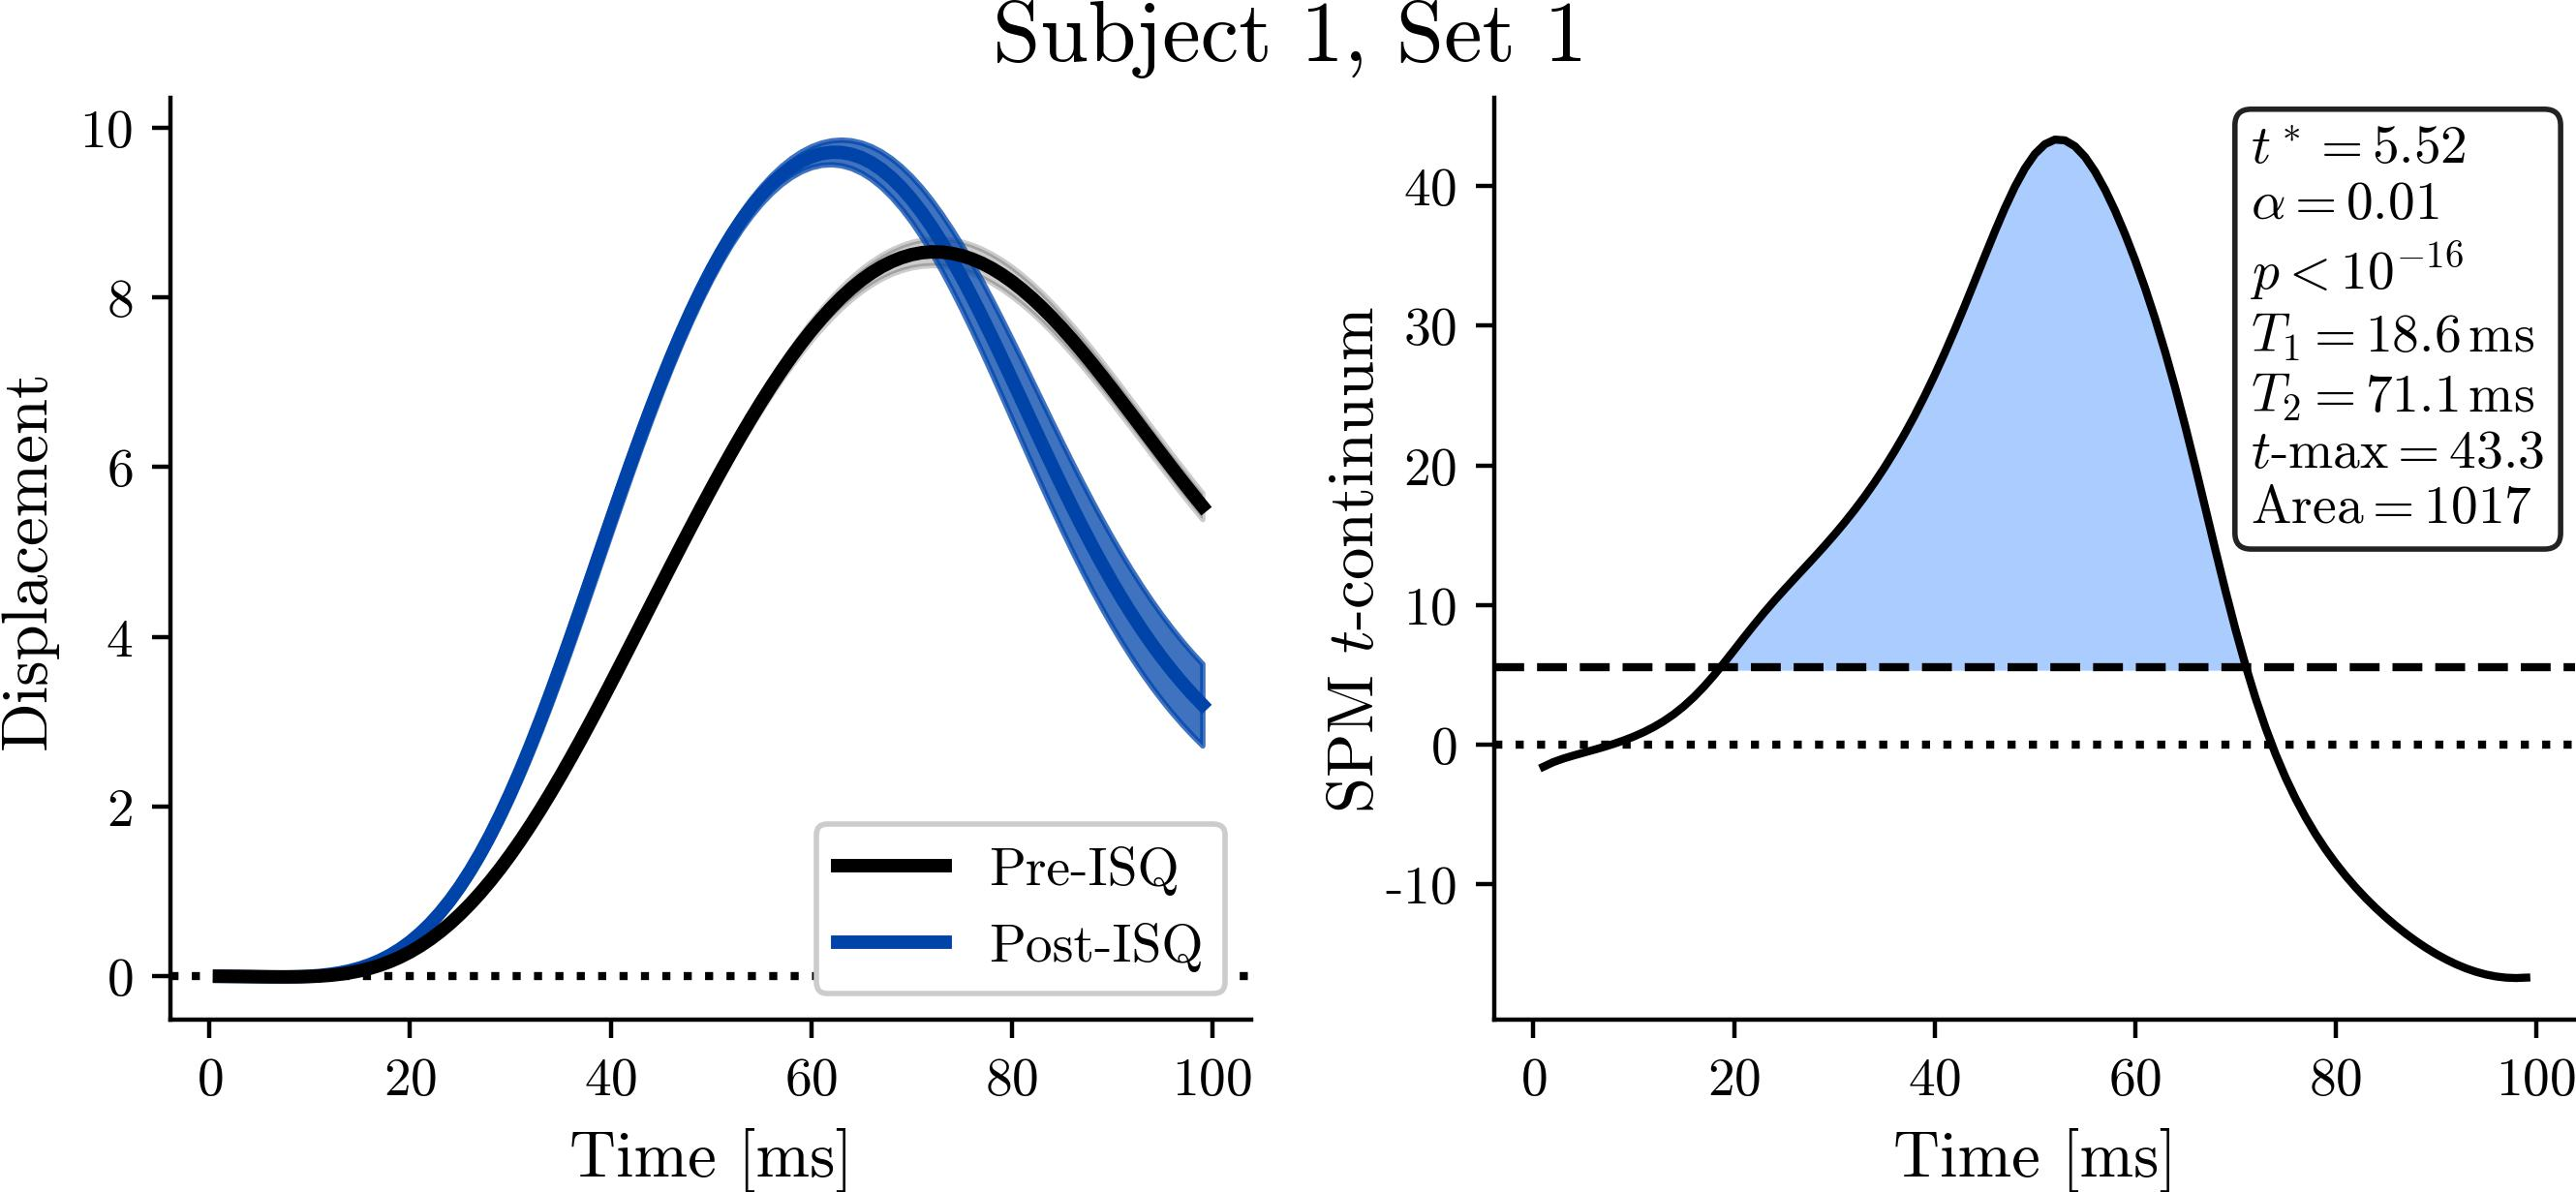
\includegraphics[width=\textwidth]{spm-plot-by-subj-by-set.jpg}
    \caption{A representative comparison of 8 pre- and 8 post-conditioning TMG signals from Subject 1's set 1.
    % TODO: correct subject name
    Mean TMG signals and their standard deviation clouds appear on the left---note the larger amplitude and faster time to peak contraction in the post-ISQ signals, indicating post-activation potentiation.
    The SPM $ t $-continuum and threshold value $ t^{*} $ from a paired SPM $ t $-test of the pre- and post-ISQ signal pairs appears on the right, together with the discrete SPM metrics defined in Section~\ref{sss:spm_analysis}.
    The large supra-threshold SPM region and low $ p $ value indicate a very small probability that differences in the pre- and post-ISQ signals arose from chance alone.}
    \label{fig:spm_example_result_by_subj_by_set}
\end{figure}

We first show a representative test comparing 8 pre-ISQ and 8 post-ISQ TMG signals from a single measurement set for one subject---this test configuration would be used in practice to identify post-activation potentiation in a given subject after a single conditioning exercise set.
A statistical comparison of the pre-ISQ and post-ISQ discrete twitch contraction parameters appears in Table~\ref{tab:tmg_params_by_subj_by_set},
and the complementary SPM comparison of the pre-ISQ and post-ISQ TMG signals is shown in Figure~\ref{fig:spm_example_result_by_subj_by_set}.

The pre-ISQ and post-ISQ TMG signals in Figure~\ref{fig:spm_example_result_by_subj_by_set} are clearly distinct even at a glance---the set of post-ISQ signals is larger in amplitude and reaches peak contraction faster than the corresponding set of pre-ISQ signals.
The associated SPM $ t $-test produces a large supra-threshold region and indicates a very low probability that the difference in the pre-ISQ and post-ISQ signals is due to chance alone.
The discrete twitch contraction parameters in Table~\ref{tab:tmg_params_by_subj_by_set} further endorse the observed potentiation-like trend of larger twitch amplitude and faster contraction following the ISQ conditioning exercise.

\begin{table}
    \centering
    \caption{A statistical comparison of pre- and post-ISQ TMG parameters from subject 1's measurement set 1.
    % TODO: correct subject name
    The twitch contraction parameters in each row were defined in Section~\ref{sss:discrete_twitch_params}.
    The columns $ \mu_{\mathrm{pre}} $ and $ \mu_{\mathrm{post}} $ show the mean value of each parameter across all eight measurements in the set, $ \sigma_{\mathrm{pre}} $ and $ \sigma_{\mathrm{post}} $ show the corresponding standard deviations, and the ``change'' column shows the percent change in each parameter relative to the pre-ISQ value.
    The $ \lvert t \rvert $ column shows the $ t $-statistic from a paired, two-tailed Student's $ t $-test comparing the (pre-ISQ, post-ISQ) pairs for each parameter, and the $ p $ column shows the associated $ p $ value.}
    \vspace{1ex}
    \renewcommand{\arraystretch}{1.2}
    \input{tables/tmg_stats_by_subj_by_set.tex}
    \label{tab:tmg_params_by_subj_by_set}
\end{table}

\subsection{Potentiation in a given subject across all conditioning sets}
Next, we show the results of comparing one pre-ISQ TMG signal from each of subject 1's eight measurement sets (for a total of eight pre-ISQ signals) to the corresponding eight post-ISQ TMG signals.
% TODO: correct subject name
This test configuration evaluates the extent to which the subject consistently produced a potentiation-like post-conditioning state in each measurement set over the course of the entire testing protocol.
A statistical comparison of pre-ISQ and post-ISQ discrete twitch contraction parameters appears in Table~\ref{tab:tmg_params_by_subj_across_sets},
and the associated SPM comparison of pre-ISQ and post-ISQ TMG signals is shown in Figure~\ref{fig:spm_example_result_by_subj_by_set}.

It is worth commenting on the larger TMG signal standard deviation clouds in Figure~\ref{fig:spm_example_result_by_subj_across_sets} relative to Figure~\ref{fig:spm_example_result_by_subj_by_set}.
This is to be expected---Figure~\ref{fig:spm_example_result_by_subj_across_sets} compares signals across eight different sets while Figure~\ref{fig:spm_example_result_by_subj_by_set} compares eight signal pairs from a single set, and it is natural to expect signals from different exercise sets to have larger variance than signals from the same exercise set due to neuromuscular adaptations between sets.
As a result of the relatively larger TMG signal variance in Figure~\ref{fig:spm_example_result_by_subj_across_sets}, the SPM paired $ t $-test produces a smaller supra-threshold cluster than in Figure~\ref{fig:spm_example_result_by_subj_by_set}, but still comfortably rejects the null hypothesis that differences in pre-ISQ and post-ISQ signals arise from chance alone.

\begin{table}
    \centering
    \caption{A statistical comparison of pre-ISQ and post-ISQ TMG parameters across measurement sets using the first measurement from each of subject 1's eight measurement sets.
    % TODO: correct subject name
    Each column has the same meaning as in Table~\ref{tab:tmg_params_by_subj_by_set}.
    Note the generally larger standard deviations in parameter values relative to Table~\ref{tab:tmg_params_by_subj_by_set}, in which parameter values all come from one set (rather than eight),
    mirroring the trend in Figures~\ref{fig:spm_example_result_by_subj_by_set} and~\ref{fig:spm_example_result_by_subj_across_sets}.}
    \vspace{1ex}
    \renewcommand{\arraystretch}{1.2}
    \input{tables/tmg_stats_by_subj_across_sets.tex}
    \label{tab:tmg_params_by_subj_across_sets}
\end{table}

\begin{figure}
	\centering
    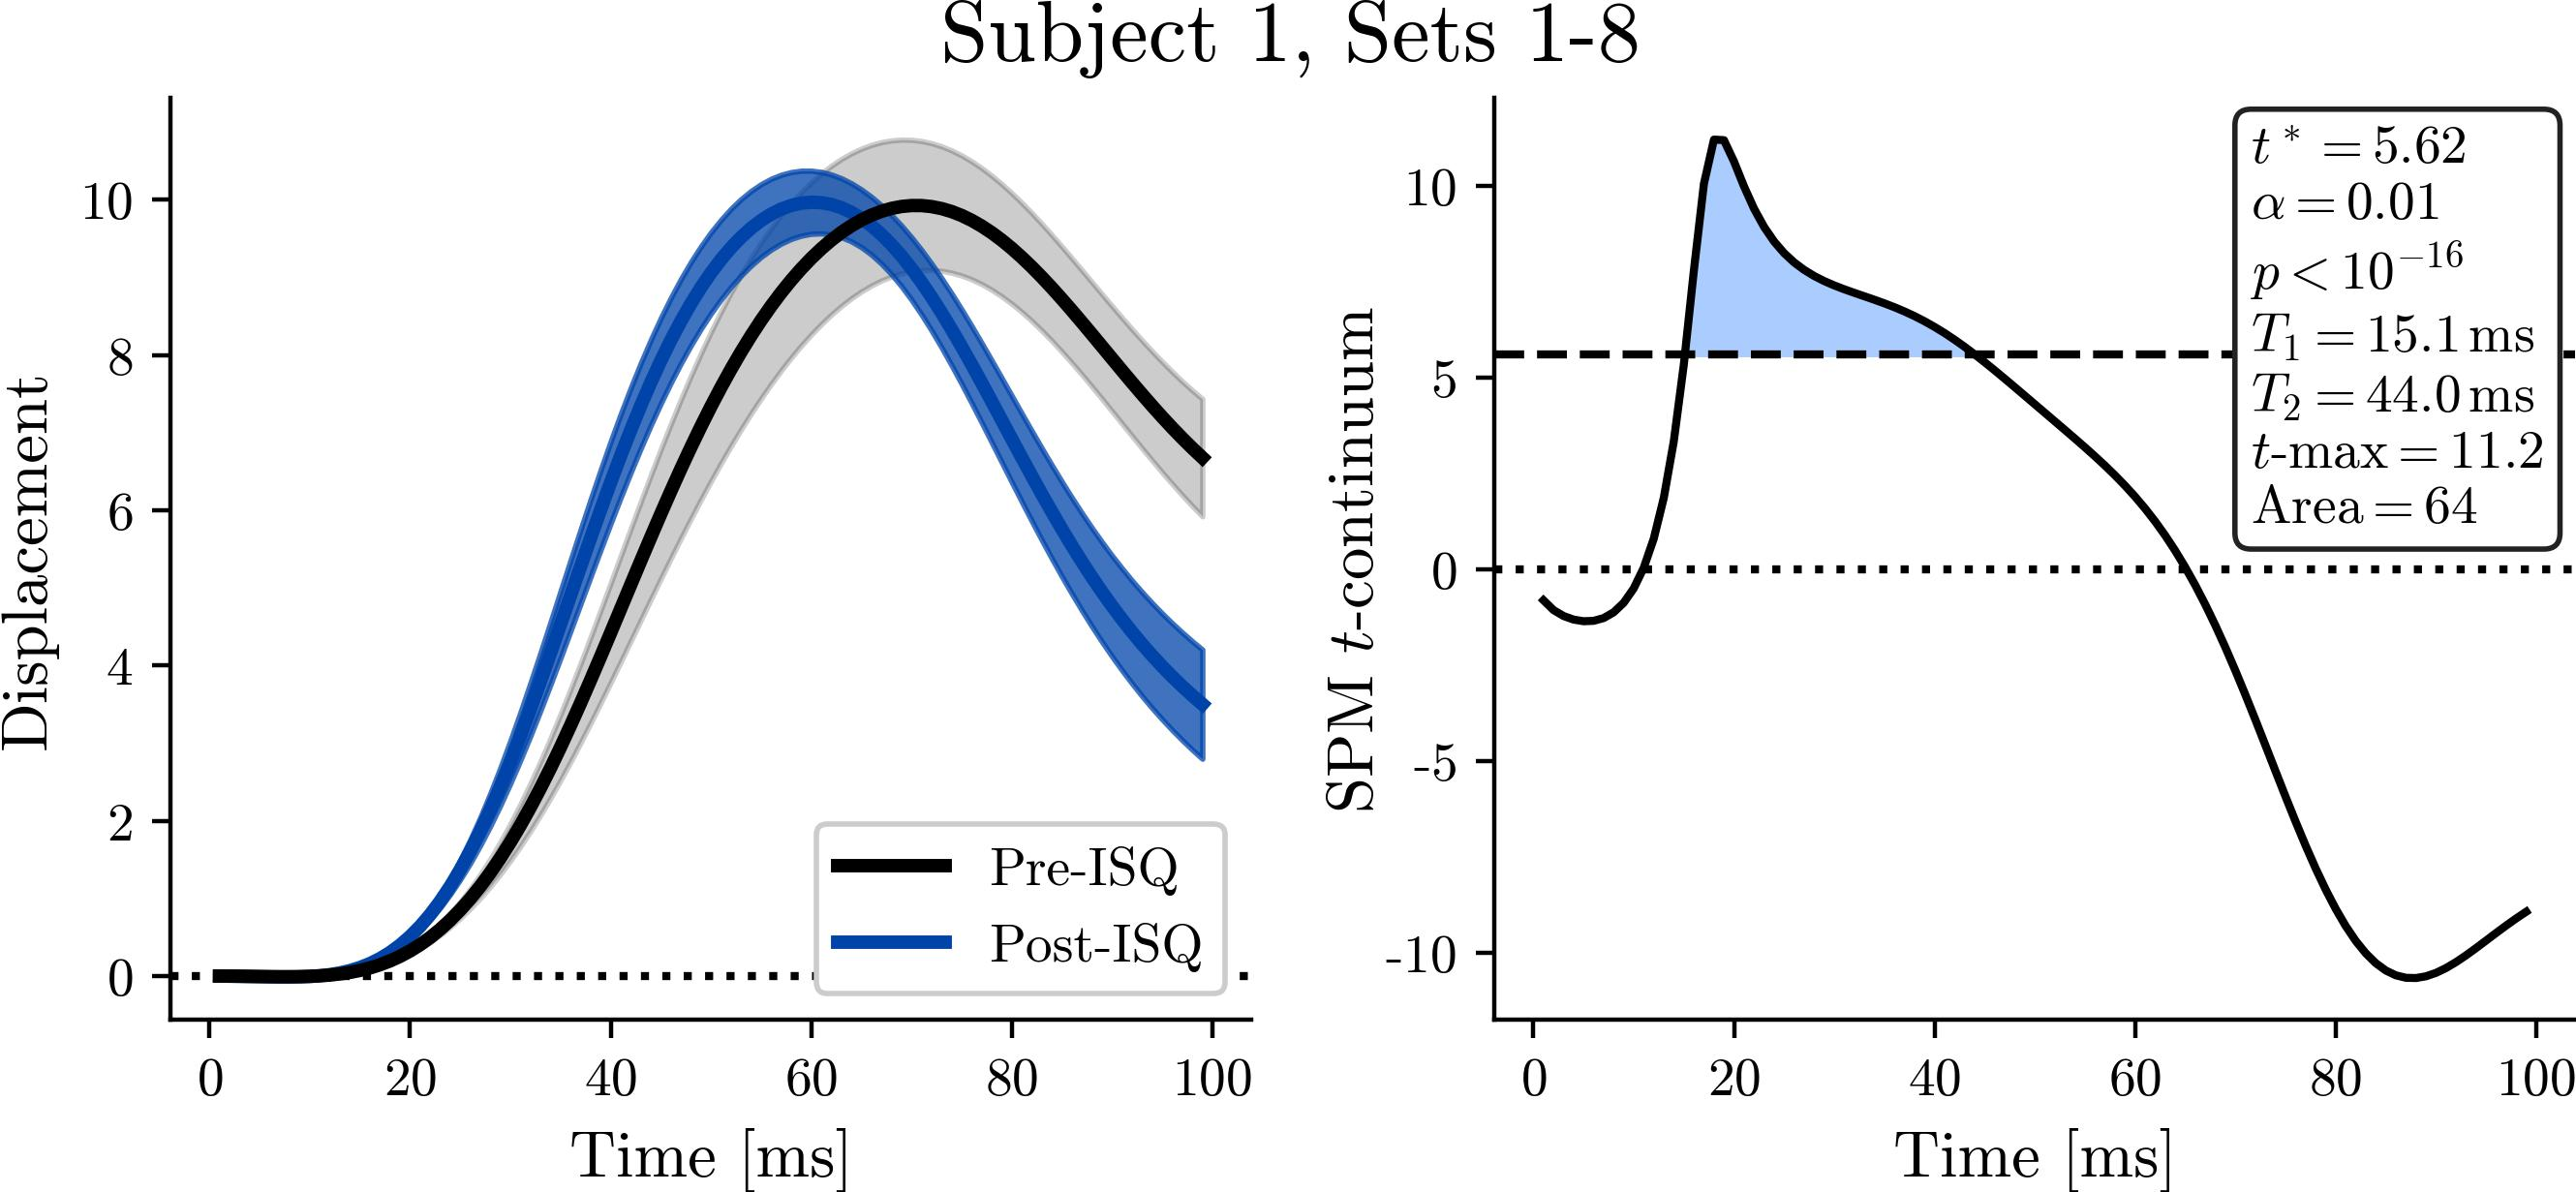
\includegraphics[width=\textwidth]{spm-plot-by-subj-across-sets.jpg}
    \caption{A representative comparison of pre- and post-conditioning TMG signals across measurement sets using the first measurement from each of subject 1's eight measurement sets.
    % TODO: correct subject name
    Mean TMG signals and their standard deviation clouds appear on the left, and the associated SPM $ t $-continuum and threshold value $ t^{*} $ on the right---see Figure~\ref{fig:spm_example_result_by_subj_by_set} for details.
    Note the larger standard deviation clouds and smaller supra-threshold region than in Figure~\ref{fig:spm_example_result_by_subj_by_set}, as a result of neuromuscular adaptations between measurement sets.}
    \label{fig:spm_example_result_by_subj_across_sets}
\end{figure}

\subsection{Potentiation across subjects for a given set}
Finally, we show the results of comparing pre- and post-ISQ TMG signals across all subjects, using one pre-ISQ and one post-ISQ TMG signal per subject per set, for a total of 54 (pre-ISQ, post-ISQ) signal pairs.
A comparison of TMG parameter values across all subjects for sets 1-4 appears in Table~\ref{tab:tmg_params_across_subj_by_set}, and each set exhibits the potentiation-like trend of larger contraction amplitude and faster contraction times, even when parameter values are averaged across all subjects.
A complementary SPM comparison of (pre-ISQ, post-ISQ) TMG signals across all subjects appears in Figure~\ref{fig:spm_example_across_subj_by_set}.
As might be expected for a comparison across all subjects, the variance in the TMG signals is quite large.
Nonetheless, in each set the SPM paired $ t $-test strongly indicates a potentiation-like trend across subjects.

\begin{table}
    \centering
    \caption{Set-by-set comparison of pre- and post-ISQ twitch contraction parameter values across all subjects---note the consistent, potentiation-like increase in muscle amplitude and decrease in contraction time following ISQ.
    See Section~\ref{sss:discrete_twitch_params} for the definition of each parameter.}
    \vspace{1ex}

    \renewcommand{\arraystretch}{1.2}
    \begin{tabular}{c}
        \input{tables/tmg_stats_across_subj_by_set_1.tex} \hfill \\
        \input{tables/tmg_stats_across_subj_by_set_2.tex} \hfill \\
        \input{tables/tmg_stats_across_subj_by_set_3.tex} \hfill \\
        \input{tables/tmg_stats_across_subj_by_set_4.tex} \hfill \\
    \end{tabular}

    \label{tab:tmg_params_across_subj_by_set}
\end{table}

\begin{figure}
	\centering
    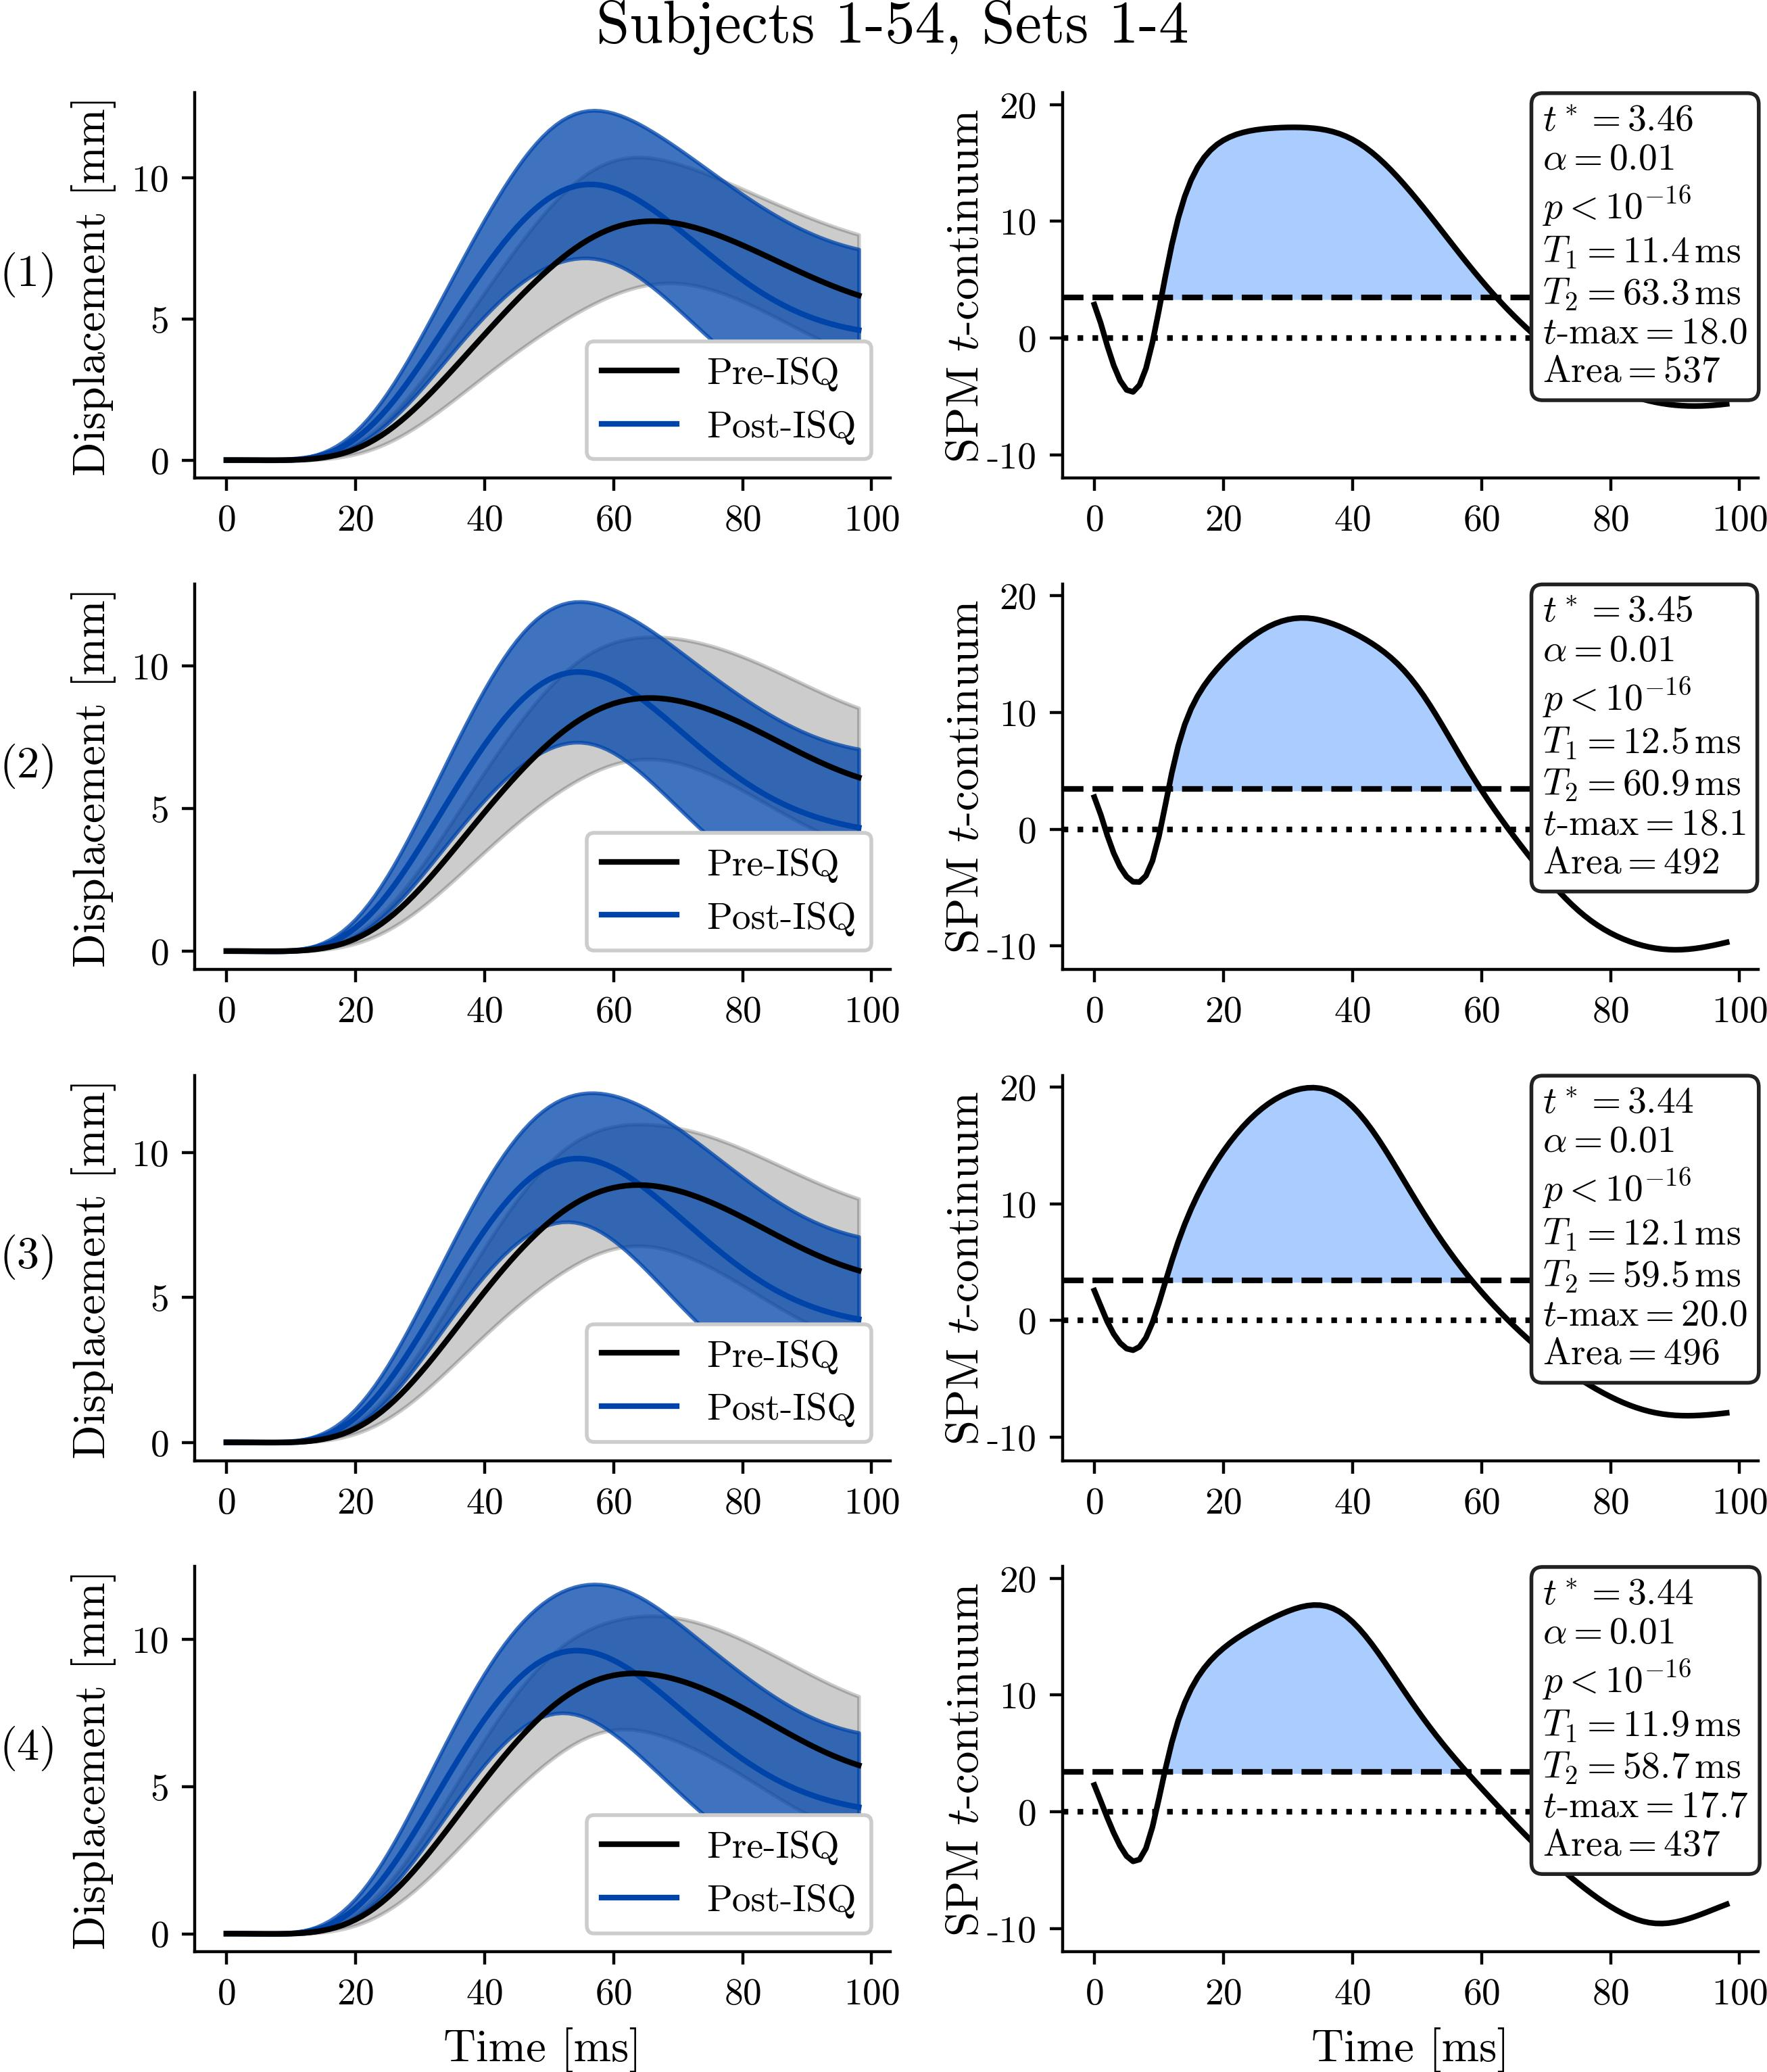
\includegraphics[width=\textwidth]{spm-plot-by-set-across-subj.jpg}
    \caption{Results of an SPM comparison of (pre-ISQ, post-ISQ) TMG signals across all subjects for measurement sets 1-4, using one (pre-ISQ, post-ISQ) signal pair from each of the 54 subjects in each set.
    Mean TMG signals and their standard deviation clouds appear on the left, and the associated SPM $ t $-continuum and threshold value $ t^{*} $ on the right---see Figure~\ref{fig:spm_example_result_by_subj_by_set} for details.
    Despite the large TMG signal variance, as might be expected for a cross-subject comparison, the SPM tests reliably detect a potentiation-like trend across all subjects, as indicated by the large supra-threshold regions and small $ p $ values.}

    \label{fig:spm_example_across_subj_by_set}
\end{figure}

\section{Discussion}
The present study aimed to assess the potential of SPM for detecting and quantifying twitch potentiation following a conditioning exercise.
We used SPM to compare TMG measurements of the rectus femoris muscle's contractile response before and after an incline squat, and found that SPM consistently distinguished between pre- and post-ISQ muscle responses (Figures~\ref{fig:spm_example_result_by_subj_by_set}, \ref{fig:spm_example_result_by_subj_across_sets}, \ref{fig:spm_example_across_subj_by_set}).

In parallel, we wished to test SPM's compatibility with the traditional approach of comparing pre- and post-conditioning values of scalar twitch contraction parameters computed retrospectively from the muscle's contractile response \citep{cochrane, kuu, wallace, rodriguez-falces}.
We paired every SPM analysis with a corresponding comparison of the scalar TMG parameters \Dm, \Td, \Tc, \RDDMax, and \RDDMaxTime (Section~\ref{sss:discrete_twitch_params}).
The results were promising.
Potentiation-like differences in scalar parameters (Tables~\ref{tab:tmg_params_by_subj_by_set}, \ref{tab:tmg_params_by_subj_across_sets}, \ref{tab:tmg_params_across_subj_by_set}) went hand in hand with SPM test results indicative of potentiation (Figures~\ref{fig:spm_example_result_by_subj_by_set}, \ref{fig:spm_example_result_by_subj_across_sets}, \ref{fig:spm_example_across_subj_by_set}), suggesting that SPM is compatible with traditional 0D comparison of scalar contraction parameters, as discussed in \cite{pataky-roi}.

SPM-based detection of potentiation builds on comparison of 0D contraction parameters by offering more interpretable and perhaps more biomechanically meaningful results.
Namely:
\begin{itemize}

    \item The result of SPM analysis---a test statistic continuum and associated significance threshold value---are directly interpretable in the time domain.
    As a consequence, the result of SPM analysis has a far more intuitive visual representation than a tabular comparison of 0D parameter values---compare any of Figures~\ref{fig:spm_example_result_by_subj_by_set}, \ref{fig:spm_example_result_by_subj_across_sets} and \ref{fig:spm_example_across_subj_by_set} to the corresponding Tables~\ref{tab:tmg_params_by_subj_by_set}, \ref{tab:tmg_params_by_subj_across_sets} and \ref{tab:tmg_params_across_subj_by_set}.
    Because the test statistic continuum is a time series just like the originally-measured muscle response, SPM also offers insight as to when a potentiation-like state occurred over the course of a muscle twitch.

    \item Computing 0D twitch contraction parameters reduces the originally-measured muscle response---generally a one-dimensional time series---to a single scalar value. 
    SPM, meanwhile, analyzes biomechanical measurements in their original time series form, which should mitigate information loss caused by preprocessing and dimensionality reduction.

\end{itemize}

\subsection{Practical use}
The SPM1D package \citep{pataky-spm1d} makes practical use of SPM relatively straightforward---the practitioner need only measure pre- and post-conditioning muscle responses and plug these measurements into test-statistic and inference functions provided by the SPM1D API, which performs all necessary computations without further work required from the user.

A practical experiment using SPM to detect PAP would proceed roughly as follows.
The practitioner, after finding a volunteer and deciding on a target muscle and conditioning exercise, first takes a set---say 5 to 10---of baseline time-series measurements of the muscle's contractile response in a pre-conditioning state.
The volunteer then performs a conditioning, followed immediately by a set of post-conditioning muscle response measurements.
Letting $ \mu_{\mathrm{pre}}(t) $ and $ \mu_{\mathrm{post}}(t) $ denote the mean pre- and post-conditioning muscle response at time $ t $, respectively, as in Equation~\ref{eq:spm_null_hypothesis},
the practitioner first assumes the null hypothesis that
\begin{equation*}
    \mu_{\mathrm{pre}} (t) - \mu_{\mathrm{post}} (t) = 0 \text{ for all } t,
\end{equation*}
interpreted loosely as differences in pre- and post-conditioning muscle responses arising from chance alone.
The pre- and post-conditioning muscle responses are then compared with an SPM test provided by the SPM1D software, yielding an SPM test statistic continuum and associated significance threshold value $ t^{*} $, as described in Section~\ref{sss:spm_analysis} and shown in Figures~\ref{fig:spm_example_result_by_subj_by_set}, \ref{fig:spm_example_result_by_subj_across_sets} and \ref{fig:spm_example_across_subj_by_set}.
Should the test statistic continuum exceed $ t^{*} $, the practitioner may reject the null hypothesis and interpret a larger-amplitude post-conditioning response as arising from PAP.

SPM, like any statistical method, must act on a set of multiple muscle contraction measurements to give meaningful results.
This imposes an experimental limitation: the set of post-conditioning measurements must be taken in rapid succession and completed in a time frame that is small in comparison with PAP's relative short ($ \sim \SI{30}{\second} $; \cite{vandervoort}) half-life.
Doing so requires a fast, repeatable measurement technique, which may involve relatively sophisticated equipment beyond the scope of in-the-field tests.

\subsection{Conclusion}
In this study, SPM consistently distinguished between pre- and post-conditioning TMG muscle responses across a variety of subjects and test configurations.
SPM appears to be a useful new tool for detecting and quantifying twitch potentiation that my be used in tandem with---or as a more intuitive and biomechanically relevant alternative to---traditional post-hoc analysis of 0D twitch contraction parameters.

% https://www.frontiersin.org/about/policies-and-publication-ethics
\section*{Conflict of Interest Statement}
The authors declare that the research was conducted in the absence of any commercial or financial relationships that could be construed as a potential conflict of interest.

\section*{Author Contributions}
The Author Contributions statement must describe the contributions of individual authors referred to by their initials and, in doing so, all authors agree to be accountable for the content of the work.
Please see \href{https://www.frontiersin.org/about/policies-and-publication-ethics#AuthorshipAuthorResponsibilities}{here} for full authorship criteria.

\section*{Funding}
Details of all funding sources should be provided, including grant numbers if applicable.
Please ensure to add all necessary funding information, as after publication this is no longer possible.

\section*{Acknowledgments}
The authors thank all the volunteers for their time and patience.

\section*{Supplemental Data}
 \href{http://home.frontiersin.org/about/author-guidelines#SupplementaryMaterial}{Supplementary Material} should be uploaded separately on submission, if there are Supplementary Figures, please include the caption in the same file as the figure. LaTeX Supplementary Material templates can be found in the Frontiers LaTeX folder.

\section*{Data Availability Statement} \label{s:data_availability}
The datasets analyzed for this study are publicly available and can be found in the [NAME OF REPOSITORY] [LINK].
% Please see the availability of data guidelines for more information, at https://www.frontiersin.org/about/author-guidelines#AvailabilityofData

\bibliographystyle{Frontiers-Harvard}
\bibliography{references}

\end{document}
